\section{Instruction Sets} 
  
  Let's review what we have so far. From only gates, we have constructed the three main components. 
  \begin{enumerate}
    \item A CPU that can do various arithmetic operations with the ALU and multiplexors. 
    \item A larger memory bank, called RAM, where the CPU can load and store to. 
    \item Since a CPU cannot directly do operations in RAM, a set of registers is built into the CPU and is the only place where the CPU can perform operations.\footnote{which is why it must move data from memory to registers before it can perform operations on it.}
  \end{enumerate}

  While this is physically implemented in hardware, it is probably not the most efficient to take pieces of wires and directly send electrical signals by physically tapping the pins on the processor. What we first need is some \textit{interface} to efficiently communicate with our machine---along with it some sort of standard that both the machine and the human can understand. This naturally introduces an \textit{instruction set}, which is a more human-friendly abstraction above the hardware level. 

  Note that the instruction set is the border between the hardware and software level. Another name for instruction sets is \textit{assembly}, which has many different types of languages depending on the type of CPU. The specific implementations of assembly languages---notably x86, ARM, and RISC-V---will be detailed in my separate assembly notes. This section is to describe the general operations that are considered essential, and we will talk about specific implementations in occasional examples. 

  \begin{definition}[Instruction Set Architecture]
    The \textbf{instruction set architecture (ISA)} of a CPU is basically a description of what it can do. It specifies the following. 
    \begin{enumerate}
      \item A predetermined set of \textbf{instructions}---also known as \textbf{opcodes}---that describes the operations that the CPU supports. 
      \item The instruction length and decoding, along with its complexity. 
      \item The performance vs power efficiency. 
    \end{enumerate}

    \begin{figure}[H]
      \centering
      \begin{subfigure}[b]{0.48\textwidth}
        \centering
        \begin{lstlisting}
          OPCODE1 arg1 arg2 arg3 
          OPCODE2 arg1 arg2
          ...
          OPCODEn arg1 
        \end{lstlisting}
        \caption{The syntax may differ across ISAs and opcodes, but it is usually the opcode followed by its arguments/operands. The specific opcodes available are usually documented in the ISA's provider page online.}
      \end{subfigure}
      \hfill 
      \begin{subfigure}[b]{0.48\textwidth}
        \centering
        \begin{lstlisting}
          0100 0010 0110 1111 
          0001 000001 010100
          ... 
          1101 1100 00000000 
        \end{lstlisting}
        \caption{Every instruction (opcode and arguments) has a direct binary representation which can entirely fit into a register. In here, we consider a register of 16 bits, and unused bits are zero-padded.}
      \end{subfigure}
      \label{fig:isa_syntax}
    \end{figure}
  \end{definition}

  Note that it only makes sense to talk about the instruction set architecture of some processing unit (e.g. CPU, GPU), and nothing more/less. It does not make sense to talk about the ISA of a computer, and it is usually implied that we are talking about the CPU residing \textit{in} the computer. The ISA is also a subset of the more general \textit{computer architecture}. 

  \begin{example}[CISC vs RISC]
    ISAs can be classified into two types. 
    \begin{enumerate} 
      \item The \textbf{complex instruction set computer} (CISC) is characterized by a large set of complex instructions, which can execute a variety of low-level operations. This approach aims to reduce the number of instructions per program, attempting to achieve higher efficiency by performing more operations with fewer instructions.
      \item The \textbf{reduced instruction set computer} (RISC) emphasizes simplicity and efficiency with a smaller number of instructions that are generally simpler and more uniform in size and format. This approach facilitates faster instruction execution and easier pipelining, with the philosophy that simpler instructions can provide greater performance when optimized.
    \end{enumerate}
  \end{example}

  The CPU executes instructions from memory one at a time and executes them, known as the \textbf{fetch-execute cycle}. It consists of 4 main operations. 
  \begin{enumerate} 
    \item \textbf{Fetch}: The \textbf{program counter}, which holds the memory address of the next instruction to be executed, tells the control unit to fetch the instruction from memory through the databus. 
    \item \textbf{Decode}: The fetched data is passed to the \textbf{instruction decoder}, which figures out what the instruction is and what it does and stores them in the registers.
    \item \textbf{Execute}: The arithmetic and logic unit then carries out these operations. 
    \item \textbf{Store}: Then it puts the results back on the databus, and stores them back into memory.
  \end{enumerate} 
  The CPU's \textbf{clock cycle} is the time it takes for the CPU to execute one instruction. More specifically, the clock cycle refers to a single oscillation of the clock signal that synchronizes the operations of the processor and the memory (e.g. fetch, decode, execute, store), and decent computers have clock cycles of at least $2.60$GHz (2.6 billion clock cycles per second). 

  We should first start off with describing the high level categories of an opcode and an operand. Like higher level programming languages, we can perform operations, do comparisons, and jump to different parts of the code. 

  \begin{definition}[Types of Instructions]
    There are generally three types of instructions. 
    \begin{enumerate} 
      \item \textbf{Data Movement}: These instructions move data between memory and registers or between the registery and registery. Memory to memory transfer cannot be done with a single instruction. 
        \begin{lstlisting} 
          %reg = Mem[address]     # load data from memory into register
          Mem[address] = %reg     # store register data into memory
        \end{lstlisting}
      \item \textbf{Arithmetic Operation}: Perform arithmetic operation on register or memory data. 
        \begin{lstlisting} 
          %reg = %reg + Mem[address]     # add memory data to register
          %reg = %reg - Mem[address]     # subtract memory data from register
          %reg = %reg * Mem[address]     # multiply memory data to register
          %reg = %reg / Mem[address]     # divide memory data from register
        \end{lstlisting}
      \item \textbf{Control Flow}: What instruction to execute next both unconditional and conditional (if statements) ones. With if statements, loops can then be defined. 
        \begin{lstlisting} 
          jmp label     # jump to label
          je label      # jump to label if equal
          jne label     # jump to label if not equal
          jg label      # jump to label if greater
          jl label      # jump to label if less
          call label    # call a function
          ret           # return from a function
        \end{lstlisting}
    \end{enumerate}
  \end{definition}

  \begin{definition}[Types of Operands]
    When we parse an instruction, its operands are one of three things. 
    \begin{enumerate}
      \item Constant values/numbers, known as \textit{literals}
      \item Registers, or more specifically, values that are currently in a register. 
      \item Memory forms, which refer to some representation of a memory addresses 
    \end{enumerate}

    These are equivalently determined by their \textbf{mode of access}:
    \begin{enumerate} 
      \item \textbf{Immediate addressing} is denoted with a \texttt{\$} sign, e.g. a constant integer data \texttt{\$1}. 
      \item \textbf{Register addressing} is denoted with a \texttt{\%} sign with the following register name, e.g. \texttt{\%rax}.
      \item \textbf{Memory addressing} is denoted with the hexadecimal address in memory, e.g. \texttt{0x034AB}.
    \end{enumerate}
  \end{definition}

  \begin{example}[Register]
    There are very specific types of registers that you should know. All of these registers are implemented for all assembly languages and are integral to the workflow of the CPU.  
    \begin{enumerate}
      \item \textbf{parameter registers} which store the parameters of a function.
      \item \textbf{Return registers} which store return values of functions. 
      \item \textbf{stack pointers} which point to the top of the stack (at the top of the current stack frame). 
      \item \textbf{frame pointers} which point to the base of the current stack frame.
      \item \textbf{instruction pointers} which point to the next instruction to be executed.
    \end{enumerate}
  \end{example}


  \begin{definition}[Instruction]
    An instruction is a single line of assembly code. It consists of some instruction followed by its (one or more) operands. The instruction is a mnemonic for a machine language operation (e.g. \texttt{mov}, \texttt{add}, \texttt{sub}, \texttt{jmp}, etc.). The \textbf{size specifier} can be appended to this instruction mnemonic to specify the size of the operands. 
    \begin{enumerate} 
      \item \textbf{b} (byte) for 1 byte 
      \item \textbf{w} (word) for 2 bytes
      \item \textbf{l} (long) for 4 bytes 
      \item \textbf{q} (quad word) for 8 bytes
    \end{enumerate}
  \end{definition}

\subsection{Data Movement}

  Registers being 8 bytes mean that we can store memory addresses, and if we can store memory addresses, we can access memory, i.e. the values at those memory addresses. There are 4 ways to do this, called \textbf{addressing modes}: immediate, normal, displacement, and indexed. 

  \begin{definition}[Immediate Addressing]
    Immediate addressing is when the operand is a constant value, used with a \$ sign. 
    \begin{equation}
      \texttt{\$val}
    \end{equation}
  \end{definition}

  \begin{definition}[Normal Addressing]
    Normal addressing is when the operand is a register, used with a \% sign and the following syntax. The parentheses are used to dereference the memory address like dereferencing a pointer in C. 
    \begin{equation}
      \texttt{(R) = Mem[Reg[R]]}
    \end{equation}
    where \texttt{R} is the register name, \texttt{Reg[R]} is the value in the register, and \texttt{Mem[Reg[R]]} is the value in the memory address pointed to by the register. 
  \end{definition}

  \begin{definition}[Displacement Addressing]
    When we have a memory address stored in a register, we can add an offset to it to access a different memory address. 
    \begin{equation}
      \texttt{D(R) = Mem[Reg[R] + D]}
    \end{equation}
    where \texttt{R} is the register name and \texttt{D} is a constant displacement that specifies offset. 
  \end{definition}

  \begin{definition}[Indexed Addressing]
    Indexed addressing gives us more flexibility, allowing us to multiply the value in the register by a constant and add it to the value in another register. The general formula is shown as the top, but there are special cases: 
    \begin{align*}
      \texttt{D(Rb, Ri, S)} && = \texttt{Mem[Reg[Rb] + S*Reg[Ri] + D]} \\ 
      \texttt{D(Rb, Ri)} && = \texttt{Mem[Reg[Rb] + Reg[Ri] + D]} \\
      \texttt{(Rb, Ri, S)} && = \texttt{Mem[Reg[Rb] + S*Reg[Ri]]} \\ 
      \texttt{(Rb, Ri)} && = \texttt{Mem[Reg[Rb] + Reg[Ri]]} \\
      \texttt{(, Ri, S)} && = \texttt{Mem[S*Reg[Ri]]} 
    \end{align*}
    where \texttt{D} is a constant displacement of 1, 2, or 4 bytes, \texttt{Rb} is the base register (can be any of 8 integer registers), \texttt{Ri} is the index register (can be any register except \texttt{rsp}), and \texttt{S} is the scale factor (1, 2, 4, or 8). 
  \end{definition}

\subsection{Arithmetic}

\subsection{Conditionals} 

  Jump. 

\subsection{Assembling}

  The process in which assembly language is converted to binary is done by an \textbf{assembler}. 

  Now unlike compiled languages, which are translated into machine code by a compiler, assembly code is translated into machine code through a two-step process. First, we \textbf{assemble} the assembly code into an \textbf{object file} by an \textbf{assembler}, and then we \textbf{link} the object file into an executable by a \textbf{linker}. Some common assemblers are \textbf{NASM} (Netwide Assembler) and \textbf{GAS/AS} (GNU Assembler), and common linkers are \textbf{ld} (GNU Linker) and \textbf{lld} (LLVM Linker), both installable with \textbf{sudo pacman -S nasm ld}. 

\subsection{Control Transfer}

  These are really the three basic functions needed to do anything in assembly, but let's talk about an important implementation called the \textbf{control transfer}. Say that you want to compute a function. 
  \begin{enumerate}
    \item Then we must retrieve the data from the memory. 
    \item We must load it into our registers in the CPU and perform some computation. 
    \item Then we must store the data back into memory. 
  \end{enumerate}

  Let’s begin with a refresher on how the call stack is managed. Recall that \texttt{\%rsp} is the stack pointer and always points to the top of the stack. The register \texttt{\%rbp} represents the base pointer (also known as the frame pointer) and points to the base of the current stack frame. The stack frame (also known as the activation frame or the activation record) refers to the portion of the stack allocated to a single function call. The currently executing function is always at the top of the stack, and its stack frame is referred to as the active frame. The active frame is bounded by the stack pointer (at the top of stack) and the frame pointer (at the bottom of the frame). The activation record typically holds local variables for a function.

  \begin{figure}[H]
    \centering 
    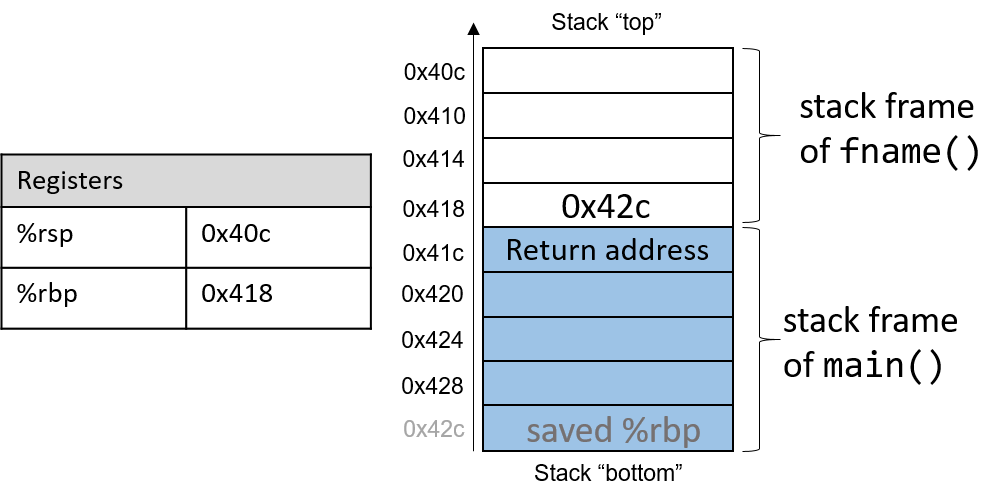
\includegraphics[scale=0.6]{img/stackFrame.png}
    \caption{The current active frame belongs to the callee function (fname). The memory between the stack pointer and the frame pointer is used for local variables. The stack pointer moves as local values are pushed and popped from the stack. In contrast, the frame pointer remains relatively constant, pointing to the beginning (the bottom) of the current stack frame. As a result, compilers like GCC commonly reference values on the stack relative to the frame pointer. In Figure 1, the active frame is bounded below by the base pointer of fname, which is stack address 0x418. The value stored at address 0x418 is the "saved" \texttt{\%rbp} value (0x42c), which itself is an address that indicates the bottom of the activation frame for the main function. The top of the activation frame of main is bounded by the return address, which indicates where in the main function program execution resumes once the callee function fname finishes executing. }
    \label{fig:stack_frame_management}
  \end{figure}


  Once we have done this we are really done. Formally, this is called Turing complete (?). 

  \begin{definition}[Control Transfers]
    We list some. 
    \begin{enumerate}
      \item Push 
      \item Pop 
      \item Call to call a function 
      \item Return to return from a function 
      \item Continue 
      \item Get out of stack with leave.  
    \end{enumerate}
  \end{definition}

  \begin{example}[Control Transfer Example]
    We show this with a minimal example with psuedocode. 
  \end{example}


  \begin{example}[Multiple Functions Example]
    Now what happens if there are multiple functions calling each other? Take a look at the following example with two functions. 
    
  \end{example}

  There is a bit of a concern here from the previous example. The main function had two functions that returned two values. As the subfunction stack frame is removed from the stack, the return value is stored in the \texttt{\%rax} register. If another function is called right after, then the return value of the second function will overwrite that of the previous one. This was not a problem in the previous example since the return value of the \texttt{assign} function was not used. However, if it was, then the return value of the \texttt{adder} function would have overwritten it. This is known as register saving. 
  \begin{enumerate}
    \item For \textbf{caller-saved registers}, the caller function is responsible for saving the value of the register before calling a function and restoring it after the function returns. The caller should save values in its stack frame before calling the callee function, e.g. by pushing all the return values of each callee in the caller stack frame. Then it will restore values after the call. 

    \begin{center}
      \textit{Therefore, if we have a set of registers $\{\texttt{\%reg}\}$, the caller must take everything and push them in the caller stack frame. Then it will restore them after the call.}
    \end{center}

    \item For \textbf{callee-saved registers}, it is the callee's responsibility to save any data in these registers before using the registers. 

      \begin{center} 
        \textit{Therefore, if we have a set of registers $\{\texttt{\%reg}\}$, then inside the callee stack frame, the callee must take everything and push them in the callee stack frame. Once it computes the final return value, then it will restore all the saved register values from the callee stack frame back into the registers for the caller to use.}
      \end{center}
  \end{enumerate}

  Ideally, we want \textit{one} calling convention to simply separate implementation details between caller and callee. In general, however, neither is best. If the caller isn't using a register, then caller-save is better, and if callee doesn't need a register, then callee-save is better. If we do need to save, then callee save generally makes smaller programs, so we compromise and use a combination of both caller-save and callee-save. 

